\section{Recommendation Quality}
\label{sec:recommendation-quality}
This section will go through the experiments that evaluate the impact of the partitioning over the recommendation quality. As explained in section \ref{sec:evaluation-pipeline} they are parameters that can be injected into the pipeline to create different experiment scenarios like choosing partitioning methods, amount of partitions, data fusion methods, evaluation metrics, number of sampled users, and the frequency of repeated recommendation for the baseline.


The experiments are done on the same machine with a hardware specification described in section \ref{subsec:hardware-spec}. Most of the tests are done with 500 sampled users. Some experiments are done with 2000 randomly sampled users to investigate the impact of sampled users on the consistency of the results. The quality of the output is then measured with the MAP@K and RBO metrics. The results measured by the RBO can be found in \ref{fig:RBO-horizontal-scaling}.


In the first section, the experiments compare a single instance with the baseline to check the reproducibility of the results. Next, the experiments determine which data fusion approach works best with a partitioning technique. Afterwards, different StarSpace models are trained and assessed. The last section scales the system horizontally and shows the recommendation quality results on four, eight, and sixteen partitions. 


\subsection{Single Machine}
\label{subsec:eval-single-machine}
The non-deterministic behavior of the random walk algorithm in generating results makes it hard to create an excellent baseline to assess the results with. To inspect the reproducibility of the results, the single partition results are compared with the generated gold standard (see section \ref{subsec:baseline-generation}). The experiments sample 500 random users and generate the objective, observed rankings on the single partition machine. The recommendation quality is measured using the Mean Average Precision at K (MAP@K), with K starting from 1 to 10. The experiments are done ten times each time using the same sampled users. 

The results of the experiments are plotted on the boxplot in figure \ref{plot:single-partition-boxplot}. Only the K values of eight, nine, and ten are shown to keep the diagram small and clear to read. As the chart denotes, the variation in each cut-off (i.e., K) is not significant. Although the non-deterministic random walk generates different recommendations each time for users, it does not impact the overall MAP@K value. So the possibility that the random walk generates the same results each time is still considered as high.


\begin{figure}[!htb]
    \centering
    \begin{tikzpicture}
	\begin{axis}[,
			boxplot/draw direction=y,
			x axis line style={opacity=0},
			axis x line*=bottom,
			xtick={1,2,3},
			xticklabels={K = 8, K = 9, K = 10},
			xtick distance=1,
			ymin=0, ymax=0.73,
			ylabel=MAP,
			height=10cm
		]
		% \addplot+ [boxplot]
		% table [y index=0] {single-partition-users-MAP-at-Ks.dat};
		% \addplot+ [boxplot]
		% table [y index=1] {single-partition-users-MAP-at-Ks.dat};
		% \addplot+ [boxplot]
		% table [y index=2] {single-partition-users-MAP-at-Ks.dat};
		% \addplot+ [boxplot]
		% table [y index=3] {single-partition-users-MAP-at-Ks.dat};
		% \addplot+ [boxplot]
		% table [y index=4] {single-partition-users-MAP-at-Ks.dat};
		% \addplot+ [boxplot]
		% table [y index=5] {single-partition-users-MAP-at-Ks.dat};
		% \addplot+ [boxplot]
		% table [y index=6] {single-partition-users-MAP-at-Ks.dat};
		\addplot+ [boxplot]
		table [y index=7] {recommendation/single-partition-users-MAP-at-Ks.dat};
		\addplot+ [boxplot]
		table [y index=8] {recommendation/single-partition-users-MAP-at-Ks.dat};
		\addplot+ [ boxplot ] 
		table [y index=9] {recommendation/single-partition-users-MAP-at-Ks.dat};
	\end{axis}
\end{tikzpicture}
    \caption{Different MAP values over ten interactions of generating recommendation with 500 users. In the experiment, the single partition results are assessed with the gold standard multiple times to investigate how far the MAP value variances.}
    \label{plot:single-partition-boxplot}
\end{figure}



The line diagram in figure \ref{plot:single-partition} shows the recommendation quality in one of the runs over the rising value of Ks for the 500 randomly sampled users. The MAP value at a cut-off of one is 90\%, indicating that the first ranked value of the 500 users is similar to the first value of the gold standard. As K increases, the ranked list gets longer, and the MAP value decreases, where at \emph{K=10} the MAP value reaches 63\%. The results highlight that the items with lower ranks in the observed ranking list differ from the gold standard values.


One may consider this as a small MAP value when comparing the results of the same machine. It is important to note that the experiment's assumption is strict, which determines that only the items in the baseline are considered relevant, and any other item beyond this baseline is irrelevant. Hypothetically, for a user, the other recommended items (i.e., items not in the baseline) could be relevant and even a better suggestion compared to the items in the baseline list. However, this can be assessed only using the user's feedback on the generated recommendations. Moreover, the applied evaluation metrics cannot measure such observation. For example, the Average Precision metric only assesses the observed ranked list with the user's baseline, and if these two lists contain different items, the computed result will be close to zero, indicating low retrieval effectiveness.

\begin{figure}[!htb]
    \centering
    \begin{tikzpicture}
	\begin{axis}[
			xlabel=K,
			ylabel=MAP,
			width=10cm,height=7cm,
			xmin=0,xmax=10.5,
			xtick distance=1,
			ymin=0,ymax=1,
			legend style={at={(1,1)},anchor=north east}
		]
				    
		\addplot[
			color=blue,
            mark=*,
            mark options={solid},
		]
		table [x=k, y=map] {recommendation/single-partition.dat};
				    
		\legend{Single Partition}
	\end{axis}
\end{tikzpicture}
    \caption{Evaluate the MAP value for increasing K for 500 users on a single instance to investigate how different the Recommendations of a single instance from the baseline items  (also generated from a single instance) are.}
    \label{plot:single-partition}
\end{figure}

\subsection{Multiple Machines}
\label{subsec:eval-multiple-machines}

\subsubsection{Data Fusion Evaluation Results}
\label{subsubsec:eval-data-fusion}
The following section will compare the recommendation quality of three data fusion methods introduced in the section \ref{sec:data-fusion-approaches} for the Murmur2 and StarSpace partitioning approaches. The main purpose of these experiments is to identify which data fusion approach produces the best single ranked list for a given partitioning method. The results are shown in the diagrams of figure \ref{plot:murmur2-data-fusion} for the Murmur2 hash partitioning method and \ref{plot:star-space-data-fusion} for the StarSpace partitioning method.


\begin{figure}[!htb]
    \centering
    \begin{subfigure}{0.8\textwidth}
        \begin{tikzpicture}
	\begin{axis}[
			xlabel=K,
			ylabel=MAP,
			width=10cm,height=7cm,
			xmin=0,xmax=10.5,
			xtick distance=1,
			ymin=0,ymax=1,
			legend style={at={(1,1)},anchor=north east}
		]
				    
		\addplot[
			color=blue,
            mark=*,
            mark options={solid},
		]
		table [x=k, y index=0] {recommendation/murmur2-data-fusion.dat};

        \addplot[
			color=red,
            mark=x,
            mark options={solid},
		]
		table [x=k, y index=1] {recommendation/murmur2-data-fusion.dat};

        \addplot[
			color=brown,
            mark=+,
            mark options={solid},
		]
		table [x=k, y index=2] {recommendation/murmur2-data-fusion.dat};
				    
		\legend{Union Results, Highest Hit, Most Interactions}
	\end{axis}
\end{tikzpicture}
        \caption{Different data fusion approaches using Murmur2 hash partitioning}
        \label{plot:murmur2-data-fusion}
    \end{subfigure}\qquad

    \begin{subfigure}{0.8\textwidth}
        \begin{tikzpicture}
	\begin{axis}[
			xlabel=K,
			ylabel=MAP,
			width=10cm,height=7cm,
			xmin=0,xmax=10.5,
			xtick distance=1,
			ymin=0,ymax=1,
			legend style={at={(1,1)},anchor=north east}
		]
				    
		\addplot[
			color=blue,
            mark=*,
            mark options={solid},
		]
		table [x=k, y index=0] {recommendation/star-space-data-fusion.dat};

        \addplot[
			color=red,
            mark=x,
            mark options={solid},
		]
		table [x=k, y index=1] {recommendation/star-space-data-fusion.dat};

        \addplot[
			color=brown,
            mark=+,
            mark options={solid},
		]
		table [x=k, y index=2] {recommendation/star-space-data-fusion.dat};
				    
		\legend{Union Results, Highest Hit, Most Interactions}
	\end{axis}
\end{tikzpicture}
        \caption{Different data fusion approaches using StarSpace partitioning}
        \label{plot:star-space-data-fusion}
    \end{subfigure}\qquad
    \caption{Comparing different data fusion approaches on two partitions for 500 sampled users. Diagram (a) shows the results of Murmur2 hash partitioning. Diagram (b) shows the results of StarSpace partitioning.}
\end{figure}


Comparing the results of the two diagrams indicates that the \emph{Union Results} approach for the Murmur2 hash and the \emph{Most Interactions} approach for StarSpace partitioning deliver the best recommendation quality. 


Looking at the chart \ref{plot:star-space-data-fusion}, it can be seen that both \emph{Union Results}, and \emph{Highest Hit} approaches deliver a weak recommendation quality. The reason for this low result is related to the data volume on the partitions and can be explained with the \emph{hit} number produced by the SALSA algorithm. 


The two approaches algorithm depends heavily on the hit number to create the single ranked list. Compared to the Murmur2 hash partitioning method, the StarSpace partitioner distributes the data much more unbalanced, creating a smaller and a bigger partition. The data distribution on two partitions with the StarSpace partitioner is illustrated on the plot \ref{plot:star-space-edge-distribution-2-partitions}. The hit count changes with the amount of data on each partition, respectively. Observing the recommendations and their hit counts on the partition with fewer data show that users with fewer interactions (i.e., vertices with a small degree) create loops in the SALSA algorithm. These loops lead the random walk to visit the same node continuously, and this will make a recommendation with a large hit number affecting the \emph{Union Results}, and \emph{Highest Hit} approaches results.


\begin{figure}[!htb]
    \centering
    \begin{tikzpicture}
	\begin{axis}[
					ybar,
					ymin=0,ymax=11884898,
					ylabel={\#Edges},
					xlabel={Hash Function},
					ytick={0,5942449,11884898},
					symbolic x coords={StarSpace},
					scaled y ticks=false,
					yticklabel style={
						/pgf/number format/fixed,
						/pgf/number format/precision=5
					},
					xtick=data,
					bar width=30,
					nodes near coords, 
					node near coords style={
						xshift=0.05cm,
						/utils/exec={\setbox0\hbox{\pgfmathprintnumber\pgfplotspointmeta}
							\pgfmathfloattomacro{\pgfplotspointmeta}{\F}{\M}{\E}
							\pgfmathsetmacro{\myanchor}{
								ifthenelse(\M*pow(10,\E-3)*2-\the\wd0>0,"east","west")
								}
						},
						rotate=90,
						anchor=\myanchor
						},
						every node near coord/.append style={
							/pgf/number format/fixed,
							/pgf/number format/precision=5
						},
						legend style={
							at={(0.5,-0.3)},
							anchor=north,legend columns=-1
						},
				]
				\addplot 
				table [y index=1, x index=0] {recommendation/star-space-edge-distribution-2-partitions.dat};
				\addplot 
				table [y index=2, x index=0] {recommendation/star-space-edge-distribution-2-partitions.dat};
				\legend{Partition 0,Partition 1}
	\end{axis}
\end{tikzpicture}
    \caption{Edge distribution of a randomly chosen StarSpace model over two partitions. The numbers on the bars indicate that the model spreads the data unevenly.}
    \label{plot:star-space-edge-distribution-2-partitions}
\end{figure}


The \emph{Most Interactions} approach works well on the StarSpace partitioning method since the model is partitioning the data based on the content of the data. This approach is not dependent on the hit number anymore and takes the partition results with the highest user degree. Having a higher degree on a partition for a user means that the user has more interactions with documents (i.e., tweets) related to each other. 


On the other hand, the \emph{Most Interactions} method does not work well for the Murmur2 hash partitioning since the data is sharded randomly and not based on the user interests. \emph{Union Results} delivers the best results for the Murmur2 hash partitioning due to its balanced distribution of data shown in the diagram \ref{plot:edge-distribution-2-partitions-murmur2}. 


The results confirm that this is a good choice to use the \emph{Most Interactions} approach with the StarSpace partitioner and \emph{Union Results} method for the Murmur2 hash partitioning method. Therefore, in the upcoming experiments for further evaluations, the combination of StarSpace partitioning with \emph{Most Interactions} data fusion method is assessed against the Murmur2 hash partitioning combined with \emph{Union Results} data fusion technique is chosen.


\subsubsection{Hyperparameter Evaluation Results}
\label{subsubsec:eval-hyperparameter}
As explained in section \ref{subsec:hyperparameter-tuning}, this thesis also investigates how different trained StarSpace models affect the partitioning of the data and, finally, the recommendation quality. Four parameters are tuned during the training. These parameters can be found in the table \ref{tab:hyperparameter}. In the following table \ref{tab:models} you will find 16 models and the parameters with which they got trained.


The hyperparameter tuning benchmark is done on a two-partition setting to keep the evaluation simple. The hyperparameter tuning experiments are structured in the following steps:

\begin{enumerate}
    \item Train the StarSpace model with the generated training dataset (see section \ref{subsec:generating-training-data}) and the parameters listed in each row of the table \ref{tab:models}.
    \item Calculate the projection matrix of the model (see section \ref{subsec:projection-matrix-calculation}).
    \item Load the model in memory and partition the test dataset on two partitions.
    \item Load sampled users (500, 2000) and generat the recommendations for each of them.
    \item Use the \emph{Most Interactions} data fusion approach to generate a single ranked list of recommendations for each user.
    \item Assess the observed ranking list with the baseline list and calculate the MAP@10.
\end{enumerate}


\begin{table}[!htb]
    \centering
    \caption{Trained model specifications}
    \label{tab:models}
    \begin{tabular}[!ht]{|l|c|c|c|c|}
        \hline
        \textbf{Model Nr.} & \textbf{Learning rate} & \textbf{Dropout probability} & \textbf{Dimensions} & \textbf{Text normalization} \\
        \hline
        \csvreader[
        late after line=\\\hline
        ]{tables/hyperparameter-models-parameters.csv}
        {
            lr=\lr, 
            dim=\dim, 
            dropoutRHS=\dropoutRHS, 
            normalizeText=\normalizeText
        }
        {
            \thecsvrow & \lr & \dropoutRHS & \dim & \normalizeText
        }%
    \end{tabular}
\end{table}


The experiments use only the \emph{Most Interactions} data fusion approach. This decision is taken with the respect to the experiments results in section \ref{subsubsec:eval-data-fusion}. This method results in a better recommendation quality compared to the other two approaches when partitioning the data with the StarSpace model. The experiments are also done once with 500 and 2000 sampled users to investigate the impact of the number of sampled users on the overall MAP@10 value.

Before diving into the recommendation quality benchmark of each model, we investigate how the different trained models impact the data (i.e., edge) distribution. The diagram \ref{plot:edge-distribution} visualizes how each model spreads the edges across two partitions. Compared to the data distribution of the Murmur2 hash partitioning method in the diagram \ref{plot:edge-distribution-2-partitions-murmur2} the partitions are uneven.


Diagram \ref{plot:hyperparameter-recommendation-quality} shows the computed mean average precision at cut-off ten for different trained models compared to the single partition and the Murmur2 hash function over 500 users. The Most interaction approach is used to unify the data together. Model 15 has the highest MAP@10 value for the merged values of two partitions among all other trained models, followed by model 7 with a value of 0.467. The chart \ref{plot:edge-distribution} shows that the data distribution of model 7 is better than model 15. In further evaluations, model 7 is used.


\begin{figure}[!htb]
    \centering
    \resizebox{0.8\textwidth}{!}{%
\begin{tikzpicture}
	\begin{axis}[
			xbar,
			xmin=0,xmax=11884898,
			height=19cm, width=13cm,
			enlarge y limits=0.05,
			xlabel={\#Edges},
			ylabel={Model Nr.},
			xtick={0,5942449,11884898},
			scaled x ticks=false,
			xticklabel style={
				/pgf/number format/fixed,
				/pgf/number format/precision=5
			},
			ytick=data,
			nodes near coords, 
			nodes near coords align={horizontal},
			every node near coord/.append style={
				/pgf/number format/fixed,
				/pgf/number format/precision=5
			},
			legend style={at={(0.5,-0.10)},
				anchor=north,legend columns=-1},
		]
		\addplot
		table [y index=0, x index=1] {recommendation/hyperparameter-edge-distribution.dat};
		\addplot 
		table [y index=0, x index=2] {recommendation/hyperparameter-edge-distribution.dat};
		\legend{Partition 0,Partition 1}
	\end{axis}
\end{tikzpicture}
}%
    \caption{Edge distribution of test dataset; sharded with different trained models over two partitions. The StarSpace models distribute the data unevenly. However, model numbers 9 and 11 keep the partitions balanced, whereas model number 8 fails to maintain balanced partitions.}
    \label{plot:edge-distribution}
\end{figure}

\begin{figure}[!htb]
    \centering
    \resizebox{0.8\textwidth}{!}{%
\begin{tikzpicture}
	\begin{axis}[
			xbar,
            xbar=5pt,
			xmin=0,xmax=1,
			height=19cm, width=13cm,
            bar width=0.1cm,
			enlarge y limits=0.03,
			xlabel={MAP@10},
			ylabel={Partitioning Method},
			xtick={0,0.25,0.5,0.75,1},
			scaled x ticks=false,
			xticklabel style={
				/pgf/number format/fixed,
				/pgf/number format/precision=5
			},
			ytick=data,
            symbolic y coords={Single,Murmur2,Model-1,Model-2,Model-3,Model-4,Model-5,Model-6,Model-7,Model-8,Model-9,Model-10,Model-11,Model-12,Model-13,Model-14,Model-15,Model-16},
			nodes near coords, 
			nodes near coords align={horizontal},
			every node near coord/.append style={
				/pgf/number format/fixed,
				/pgf/number format/precision=3,
                font=\footnotesize
			},
			legend style={at={(0.5,-0.09)},
				anchor=north,legend columns=-1},
		]
		\addplot
		table [y index=0, x index=1] {recommendation/hyperparameter-map-at-10.dat};

		\addplot[red, fill=red!30!white, x filter/.expression={x==0 ? nan : x}]
		table [y index=0, x index=2] {recommendation/hyperparameter-map-at-10.dat};

        \addplot[brown, fill=brown!30!white, x filter/.expression={x==0 ? nan : x}]
		table [y index=0, x index=3] {recommendation/hyperparameter-map-at-10.dat};

		\legend{Partition 0,Partition 1, most interactions}
	\end{axis}
\end{tikzpicture}
}%
    \caption{Comparing recommendation quality of different partitioning methods and models for 500 users. The results of the StarSpace models outperform the baseline partitioning method (Murmur2). Model 15 delivers a 30\% improvement, compared to the Murmur2 result.}
    \label{plot:hyperparameter-recommendation-quality}
\end{figure}


Another promising finding is that the text normalization does not impact the overall recommendation quality. On the other hand, it influences the data distribution on each partition. When comparing the edge distribution of models 7 and 8 in the diagram \ref{plot:star-space-edge-distribution-2-partitions}, which only differ in the text normalization parameter, we can determine that model 7 is delivering an equal distribution on two partitions. Thus, the text normalization is set to false. 


The tweets data set explains why trained models with no text normalization are delivering a better performance than those with text normalization enabled. The tweets are noisy and contain emojis and special characters that do not land in any of the text normalization buckets (see section \ref{subsubsec:star-space-text-normalization}). Therefore, the text normalization delivers a bad performance on this specific dataset.


As explained in the begining of this section the hyperparameter tests are also done over 2000 users to investigate the consistency of the results and if the number of sampled users affects the overall MAP value. The experiments do not significantly increase or decrease in the overall MAP value in each model and partitioning method. This can be seen in the chart \ref{plot:hyperparameter-recommendation-quality-2000-users}. Therefore all other experiments are done over 500 sampled users.

\begin{figure}[!htb]
    \centering
    \begin{tikzpicture}
	\begin{axis}[
			xbar,
            xbar=5pt,
			xmin=0,xmax=1,
			height=19cm, width=13cm,
            bar width=0.1cm,
			enlarge y limits=0.03,
			xlabel={MAP@10},
			ylabel={Partitioning Method},
			xtick={0,0.25,0.5,0.75,1},
			scaled x ticks=false,
			xticklabel style={
				/pgf/number format/fixed,
				/pgf/number format/precision=5
			},
			ytick=data,
            symbolic y coords={Single,Murmur2,Model-1,Model-2,Model-3,Model-4,Model-5,Model-6,Model-7,Model-8,Model-9,Model-10,Model-11,Model-12,Model-13,Model-14,Model-15,Model-16},
			nodes near coords, 
			nodes near coords align={horizontal},
			every node near coord/.append style={
				/pgf/number format/fixed,
				/pgf/number format/precision=3,
                font=\footnotesize
			},
			legend style={at={(0.5,-0.09)},
				anchor=north,legend columns=-1},
		]
		\addplot
		table [y index=0, x index=1] {recommendation/hyperparameter-map-at-10-2000-users.dat};

		\addplot[red, fill=red!30!white, x filter/.expression={x==0 ? nan : x}]
		table [y index=0, x index=2] {recommendation/hyperparameter-map-at-10-2000-users.dat};

        \addplot[brown, fill=brown!30!white, x filter/.expression={x==0 ? nan : x}]
		table [y index=0, x index=3] {recommendation/hyperparameter-map-at-10-2000-users.dat};

		\legend{Partition 0,Partition 1,highest interest}
	\end{axis}
\end{tikzpicture}
    \caption{Comparing recommendation quality of different partitioning methods and models for 2000 users to investigate the consistency of the results. The results indicate consistency of the results.}
    \label{plot:hyperparameter-recommendation-quality-2000-users}
\end{figure}


\subsubsection{Partition Request Load}
\label{subsubsec:partition-request-load}
The results of the experiments with the StarSpace model number 7 (refer to table \ref{tab:models}, and the diagrams \ref{plot:hyperparameter-recommendation-quality}, \ref{plot:star-space-edge-distribution-2-partitions}) combined with the \emph{Most Interactions} data fusion approach point out two important findings: First, this combination delivers the most similar recommendations to the baseline. Second, compared to the other trained models, this model keeps the two partition balance.


One might say that the data fusion module might only choose the recommendations list from a partition containing more data. Since the possibility that the users on a partition with more data have a significant degree number is higher. Although this hypothesis is intuitive, the measurements in the diagram \ref{subsubsec:partition-request-load} highlight that the load is almost equally balanced. Approximately 43\% of the generated recommendations list is chosen from partition zero and 57\% from partition one.

The results confirm that this is a good choice for applying the load balancer idea (see section \ref{sec:load-balancing}). The load balancer can forward the load almost equally between the two partitions.

\begin{figure}[!htb]
    \centering
    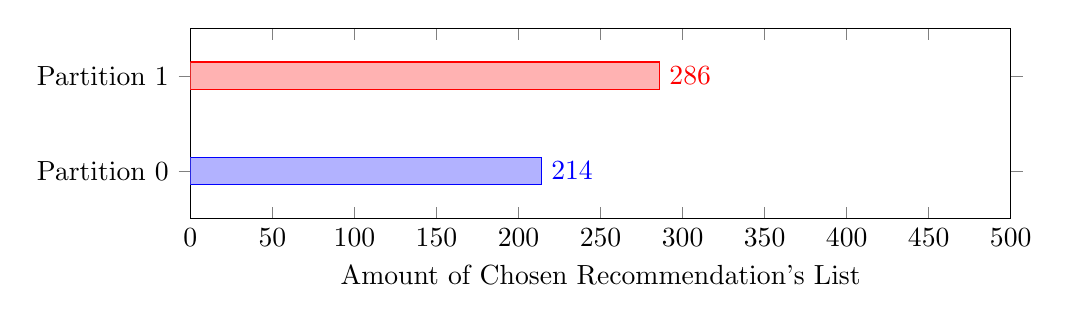
\begin{tikzpicture}
    \begin{axis}[
        xbar, 
        xmin=0, xmax=500,
        width=12cm, height=4cm, enlarge y limits=0.5,
        xlabel={Amount of Chosen Recommendation's List},
        ytick={0, 1},
        yticklabels={Partition 0, Partition 1},
        nodes near coords, nodes near coords align={horizontal},
        every axis plot/.append style={
            xbar,
            bar shift=0pt,
        }
    ]
        \addplot coordinates {(214, 0)};
        \addplot coordinates {(286, 1)};
    \end{axis}
\end{tikzpicture}

    \caption{Proportion of requests on each partition the data fusion module (with the \emph{Most Interactions} approach) makes to unify the results.}
    \label{plot:request-distribution}
\end{figure}


\subsubsection{Horizontal Scalling}
\label{subsubsec:eval-horizontal-scalling}
The previous experiments were done on two partitions to compare different partitioning methods and data fusion approaches. The following section will discuss how the number of partitions affects the recommendation quality. In other words, how the recommendation quality will change when we scale the system horizontally. The experiments are done with 500 randomly sampled users using the Murmur2 hash partitioning and the StarSpace model number 7 (refer to the table \ref{tab:models}); with data fusion approaches \emph{Union Results} and \emph{Most Interactions} respectively.


The results of the evaluations are illustrated on the plots in figure \ref{fig:horizontal-scaling}. As the plots denote, the overall MAP value decreases whenever the number of partitions grows. This decrease is because the amount of data declines on each partition, creating a sparse bipartite graph. The random walk fails to produce sound recommendations due to fewer items on each partition for the users. By increasing the amount of data, the partitions can generate better recommendations. 


In the original paper of GraphJet, the authors keep a bipartite graph with $10^9$ edges on a machine with 30~GB memory \cite{sharmaGraphJetRealtimeContent2016}. Distributing this amount of interactions among their edges on 16 devices or more can help reduce the memory needed for maintaining the bipartite graph on a single machine and help to improve the computation speed of the random walk algorithm. These improvements are penalized by the recommendation quality, but with the current measuremnts it is hard to justify such conclusion.


\begin{figure}[!htb]
	\centering
	\begin{subfigure}[b]{0.5\linewidth}
	  \centering
	  \begin{tikzpicture}
	\begin{axis}[
			xlabel=K,
			ylabel=MAP,
			width=7cm,height=7cm,
			xmin=0,xmax=10.5,
			xtick distance=1,
			ymin=0,ymax=1,
			legend style={
                at={(0.5,-0.2)},
			    anchor=north,legend columns=-1
            },
            legend columns=3,
            transpose legend
            ]
				    
		\addplot[
			color=blue,
            mark=*,
            mark options={solid},
		]
		table [x=k, y index=0] {recommendation/2-partitions.dat};
        \addlegendentry{Single Partition}

        \addplot[
			color=red,
            mark=x,
            mark options={solid},
		]
		table [x=k, y index=1] {recommendation/2-partitions.dat};
        \addlegendentry{Murmur2 Union Results}

        \addplot[
			color=brown,
            mark=+,
            mark options={solid},
		]
		table [x=k, y index=2] {recommendation/2-partitions.dat};		    
		\addlegendentry{StarSpace Most Interactions}
	\end{axis}
\end{tikzpicture}
	  \caption{2 Partitions} 
	  \label{fig:horizontal-scaling-2-partitions-a} 
	  \vspace{1cm}
	\end{subfigure}%% 
	\begin{subfigure}[b]{0.5\linewidth}
	  \centering
	  \begin{tikzpicture}
	\begin{axis}[
			xlabel=K,
			% ylabel=MAP,
			width=7cm,height=7cm,
			xmin=0,xmax=10.5,
			xtick distance=1,
			ymin=0,ymax=1,
			legend style={
                at={(0.5,-0.2)},
			    anchor=north,legend columns=-1
            },
            legend columns=3,
            transpose legend
            ]
				    
		\addplot[
			color=blue,
            mark=*,
            mark options={solid},
		]
		table [x=k, y index=0] {recommendation/4-partitions.dat};
        \addlegendentry{Single Partition}

        \addplot[
			color=red,
            mark=x,
            mark options={solid},
		]
		table [x=k, y index=1] {recommendation/4-partitions.dat};
        \addlegendentry{Murmur2 Union Results}

        \addplot[
			color=brown,
            mark=+,
            mark options={solid},
		]
		table [x=k, y index=2] {recommendation/4-partitions.dat};		    
		\addlegendentry{StarSpace Most Interactions}
	\end{axis}
\end{tikzpicture}
	  \caption{4 Partitions} 
	  \label{fig:horizontal-scaling-4-partitions-b} 
	  \vspace{1cm}
	\end{subfigure} 
	\begin{subfigure}[b]{0.5\linewidth}
	  \centering
	  \begin{tikzpicture}
	\begin{axis}[
			xlabel=K,
			ylabel=MAP,
			width=7cm,height=7cm,
			xmin=0,xmax=10.5,
			xtick distance=1,
			ymin=0,ymax=1,
			legend style={
                at={(0.5,-0.2)},
			    anchor=north,legend columns=-1
            },
            legend columns=3,
            transpose legend
            ]
				    
		\addplot[
			color=blue,
            mark=*,
            mark options={solid},
		]
		table [x=k, y index=0] {recommendation/8-partitions.dat};
        \addlegendentry{Single Partition}

        \addplot[
			color=red,
            mark=x,
            mark options={solid},
		]
		table [x=k, y index=1] {recommendation/8-partitions.dat};
        \addlegendentry{Murmur2 Union Results}

        \addplot[
			color=brown,
            mark=+,
            mark options={solid},
		]
		table [x=k, y index=2] {recommendation/8-partitions.dat};		    
		\addlegendentry{StarSpace Most Interactions}
	\end{axis}
\end{tikzpicture}
	  \caption{8 Partitions} 
	  \label{fig:horizontal-scaling-8-partitions-c} 
	\end{subfigure}%%
	\begin{subfigure}[b]{0.5\linewidth}
	  \centering
	  \begin{tikzpicture}
	\begin{axis}[
			xlabel=K,
			% ylabel=MAP,
			width=7cm,height=7cm,
			xmin=0,xmax=10.5,
			xtick distance=1,
			ymin=0,ymax=1,
			legend style={
                at={(0.5,-0.2)},
			    anchor=north,legend columns=-1
            },
            legend columns=3,
            transpose legend
            ]
				    
		\addplot[
			color=blue,
            mark=*,
            mark options={solid},
		]
		table [x=k, y index=0] {recommendation/16-partitions.dat};
        \addlegendentry{Single Partition}

        \addplot[
			color=red,
            mark=x,
            mark options={solid},
		]
		table [x=k, y index=1] {recommendation/16-partitions.dat};
        \addlegendentry{Murmur2 Union Results}

        \addplot[
			color=brown,
            mark=+,
            mark options={solid},
		]
		table [x=k, y index=2] {recommendation/16-partitions.dat};		    
		\addlegendentry{StarSpace Most Interactions}
	\end{axis}
\end{tikzpicture}
	  \caption{16 Partitions} 
	  \label{fig:horizontal-scaling-16-partitions-d} 
	\end{subfigure} 
	\caption{Recommendation quality when scaling horizontally}
	\label{fig:horizontal-scaling} 
\end{figure}
